\section{Benchmark Test Fonksiyonları}
Bu başlık altında incelenen test fonksiyonlarına ait python kodlarına \href{https://github.com/btayfur/structural-optimization/blob/main/Code/Sources/OptimizationBenchmarks}{bağlantıdan} ulaşılabilir. \sidenote{
    
\qrcode[height=1in]{https://github.com/btayfur/structural-optimization/blob/main/Code/Sources/OptimizationBenchmarks}}

Optimizasyon algoritmalarının performansını değerlendirmek ve karşılaştırmak için kullanılan standart test fonksiyonları\sidenote{Test fonksiyonları, algoritmaların güçlü ve zayıf yönlerini ortaya çıkarmada önemli rol oynar. Bir algoritmanın gerçek dünya problemlerindeki başarısı, önce bu test fonksiyonları üzerinde değerlendirilir.}, farklı zorluk derecelerine sahip matematiksel yapılar olarak karşımıza çıkar. Bu test fonksiyonları, bilinen global minimum noktaları, karmaşık yerel minimum yapıları ve çeşitli topolojik özellikleri ile algoritmaları sınamak için tasarlanmıştır.

\subsection{Benchmark Fonksiyonlarının Optimizasyondaki Rolü}

Optimizasyon algoritmalarının performansını değerlendirmek için standart test fonksiyonları kullanılır. Bu fonksiyonlar şu açılardan önem taşır:

\begin{itemize}
    \item \textbf{Karşılaştırılabilirlik:} Farklı algoritmaların aynı problem üzerindeki başarısını objektif olarak değerlendirmeyi sağlar.
    \item \textbf{Güçlü ve Zayıf Yönleri Belirleme:} Algoritmaların hangi tür problemlerde iyi performans gösterdiğini, hangi tür problemlerde zorlandığını gösterir.
    \item \textbf{Algoritma Geliştirme:} Yeni optimizasyon algoritmalarının geliştirilmesi ve iyileştirilmesi sürecinde rehberlik eder.
    \item \textbf{Gerçek Dünya Uygulamalarına Hazırlık:} Algoritmaların daha karmaşık gerçek dünya problemlerine uygulanmadan önce test edilmesini sağlar.
\end{itemize}

İdeal bir benchmark fonksiyonu, gerçek dünyadaki optimizasyon problemlerinin karmaşıklığını yansıtırken, matematiksel olarak anlaşılabilir ve analiz edilebilir olmalıdır. Benchmark fonksiyonları genellikle şu özelliklere göre sınıflandırılır: doğrusallık, modalite (tepe nokta sayısı), süreklilik, türevlenebilirlik, sınırlılık ve boyutsallık.

\subsubsection{Benchmark Fonksiyonlarının Ortak Özellikleri}

Çoğu benchmark fonksiyonu aşağıdaki özelliklere sahiptir:

\begin{itemize}
    \item Bilinen global minimum değeri ve konumu
    \item Matematiksel olarak tanımlanmış yapı
    \item Ayarlanabilir boyut (genellikle çok boyutlu uzaylara genişletilebilir)
    \item Çeşitli zorluklar (örn. yerel minimumlar, düz bölgeler, dik vadiler)
    \item Önerilen arama aralıkları
\end{itemize}

\subsection{Çok Modlu ve Tek Modlu Test Fonksiyonları}

Test fonksiyonları, içerdikleri tepe noktası (mod) sayısına göre tek modlu (unimodal) ve çok modlu (multimodal) olarak ikiye ayrılır.

\subsubsection{Tek Modlu Fonksiyonlar}

Tek modlu fonksiyonlar, yalnızca bir tane global minimuma sahiptir ve genellikle daha basit yapıdadır. Bu fonksiyonlar, algoritmanın yakınsama hızını ve hassasiyetini test etmek için kullanılır. Örnek olarak:

\begin{itemize}
    \item \textbf{Sphere Fonksiyonu:} Matematiksel olarak en basit optimizasyon test fonksiyonudur ve şu şekilde tanımlanır:
    \begin{equation}
        f(\mathbf{x}) = \sum_{i=1}^{n} x_i^2
    \end{equation}
    Global minimum $f(\mathbf{x}^*) = 0$, $\mathbf{x}^* = (0, 0, \ldots, 0)$ noktasında yer alır.
    
    \item \textbf{Booth Fonksiyonu:} İki boyutlu, çanak şeklinde bir fonksiyondur:
    \begin{equation}
        f(x, y) = (x + 2y - 7)^2 + (2x + y - 5)^2
    \end{equation}
    Global minimum $f(1, 3) = 0$ noktasındadır.
\end{itemize}

\subsubsection{Çok Modlu Fonksiyonlar}

Çok modlu fonksiyonlar, birden fazla yerel minimuma sahiptir ve bu nedenle algoritmaların yerel minimumlara takılmadan global minimumu bulabilme yeteneğini test eder. Bu fonksiyonlar, özellikle metasezgisel ve evrimsel algoritmaların performansını değerlendirmek için önemlidir. Önemli örnekler arasında:

\begin{itemize}
    \item \textbf{Ackley Fonksiyonu:} Çok sayıda yerel minimumu olan karmaşık bir test fonksiyonudur. Matematiksel olarak şöyle tanımlanır:
    \begin{equation}
        f(\mathbf{x}) = -20\exp\left(-0.2\sqrt{\frac{1}{n}\sum_{i=1}^{n}x_i^2}\right) - \exp\left(\frac{1}{n}\sum_{i=1}^{n}\cos(2\pi x_i)\right) + 20 + e
    \end{equation}
    
    Bu fonksiyonun global minimumu $f(\mathbf{x}^*) = 0$, $\mathbf{x}^* = (0, 0, \ldots, 0)$ noktasında bulunur. Genellikle $[-32.768, 32.768]$ aralığında tanımlanır.
    
    \item \textbf{Rastrigin Fonksiyonu:} Sinüzoidal modülasyonu ile çok sayıda yerel minimuma sahip zorlayıcı bir fonksiyondur:
    \begin{equation}
        f(\mathbf{x}) = 10n + \sum_{i=1}^{n} \left[ x_i^2 - 10\cos(2\pi x_i) \right]
    \end{equation}
    Global minimum $f(\mathbf{x}^*) = 0$, $\mathbf{x}^* = (0, 0, \ldots, 0)$ noktasındadır.
\end{itemize}

\begin{figure}[h]
    \centering
    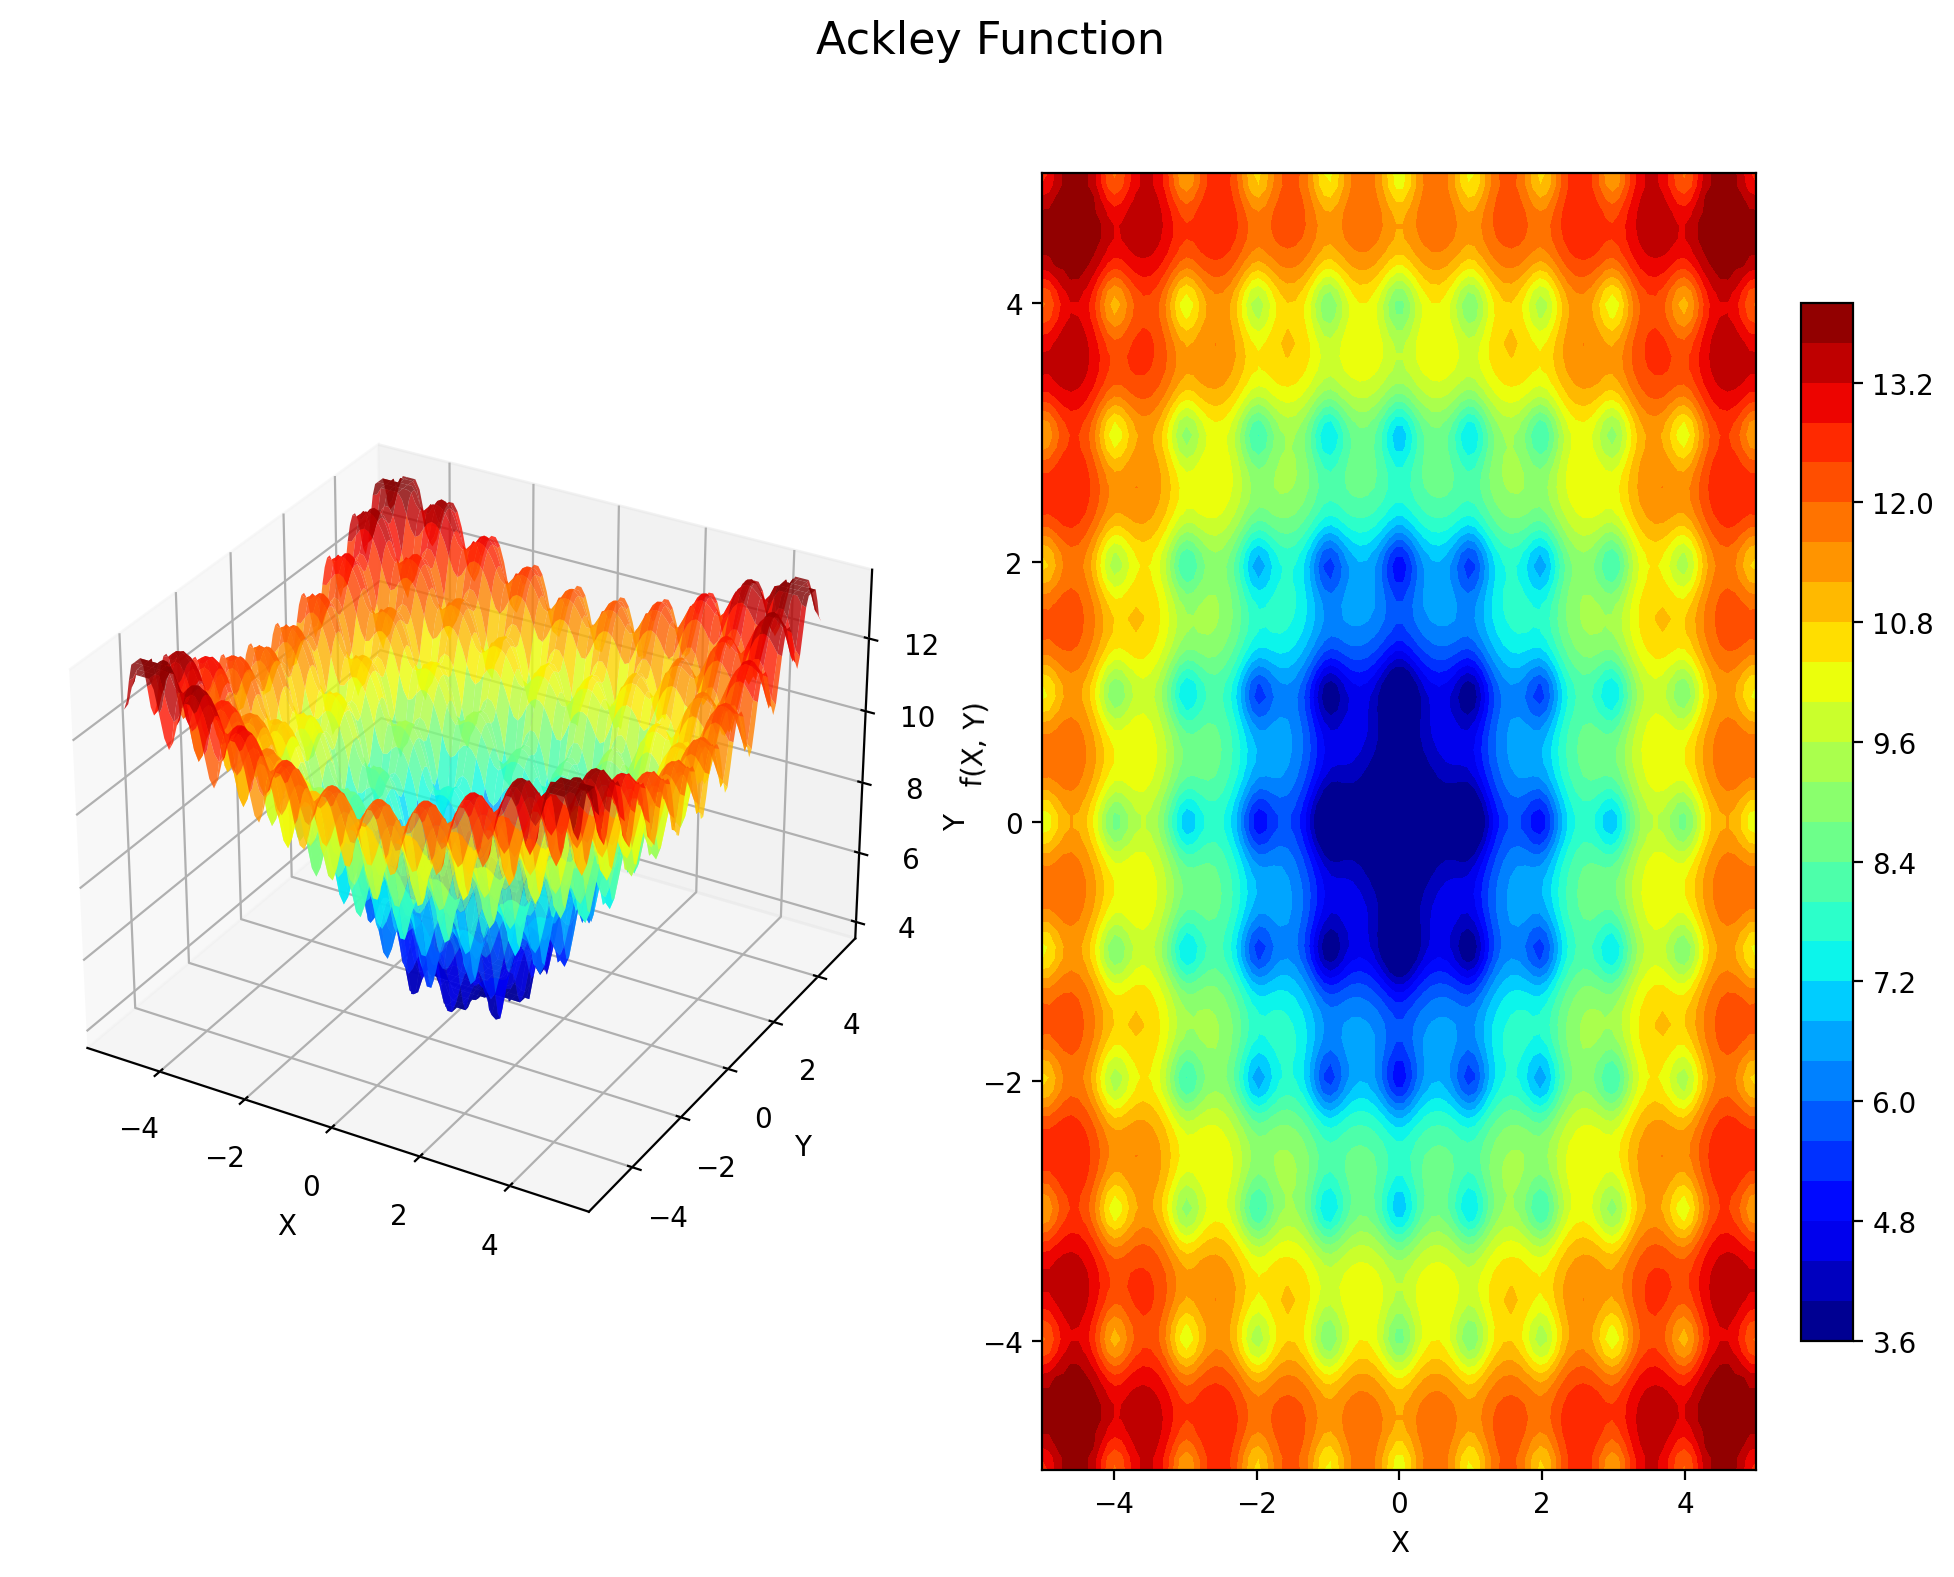
\includegraphics[width=0.8\textwidth]{weeks_new/imgs/ackley_function.png}
    \caption{Ackley fonksiyonunun 3B gösterimi (soldaki) ve kontur grafiği (sağdaki). Fonksiyonun merkezde bir global minimum ve etrafında çok sayıda yerel minimum içeren yapısı dikkat çekicidir.}
    \label{fig:ackley}
\end{figure}

\subsubsection{Ackley Fonksiyonu: Derinlemesine İnceleme}

Ackley fonksiyonu, David Ackley tarafından 1987 yılında önerilmiş ve optimizasyon algoritmaları için standart bir test fonksiyonu haline gelmiştir. Fonksiyonun matematiksel yapısı şu özellikleri ortaya çıkarır:

\begin{itemize}
    \item \textbf{Neredeyse düz bölgeler:} Merkezden uzaklaştıkça fonksiyon neredeyse düz bir yapıya sahiptir, bu da gradyan tabanlı yöntemlerin doğru yönü belirlemesini zorlaştırır.
    
    \item \textbf{Periyodik dalgalanmalar:} Kosinüs terimi nedeniyle, fonksiyon yüzeyi düzenli aralıklarla iniş ve çıkışlar gösterir, çok sayıda yerel minimum oluşturur.
    
    \item \textbf{Merkezdeki derin çukur:} Global minimum etrafında dik bir çukur bulunur, bu da algoritmanın optimuma yakın olduğunda hassas adımlar atmasını gerektirir.
\end{itemize}

Ackley fonksiyonu, özellikle şu tür algoritmaların test edilmesinde etkilidir:

\begin{itemize}
    \item Yerel aramayla global arama stratejilerini dengeleyen metasezgisel algoritmalar
    \item Çok sayıda yerel minimumdan kaçabilme yeteneğine sahip algoritmalar
    \item Farklı çözüm bölgelerini aynı anda keşfedebilen popülasyon tabanlı algoritmalar
\end{itemize}

$n$-boyutlu Ackley fonksiyonunun optimizasyonu şu zorlukları içerir:
\begin{itemize}
    \item Boyut arttıkça yerel minimum sayısı üstel olarak artar
    \item Merkeze yakın bölgelerde yüksek hassasiyet gerektirir
    \item Düz bölgelerde gradyan bilgisi yetersiz kalır
\end{itemize}

\begin{tcolorbox}[title=Ackley Fonksiyonu Optimizasyon Zorluğu]
Ackley fonksiyonu, hem keşif (exploration) hem de yararlanma (exploitation) özelliklerini aynı anda test eder:
\begin{itemize}
    \item Keşif: Geniş, neredeyse düz bölgelerde doğru yönü bulabilme
    \item Yararlanma: Merkezdeki dik çukurda hassas ayarlamaları yapabilme
    \item Denge: Yerel minimumlardan kaçarken global minimuma yakınsayabilme
\end{itemize}
\end{tcolorbox}

\subsection{Yüksek Boyutlu Optimizasyon Problemleri}

\subsubsection{Boyut Artışının Etkileri}
\begin{itemize}
    \item Arama uzayı üstel olarak büyür
    \item Hesaplama maliyeti artar
    \item Lokal minimum sayısı artar
    \item Yakınsama zorlaşır
\end{itemize}

Yüksek boyutlu optimizasyon problemleri, gerçek dünyadaki birçok mühendislik uygulamasında karşımıza çıkar. Boyut artışı, "boyutun laneti" (curse of dimensionality) olarak bilinen fenomene yol açar. Bu fenomen, boyut arttıkça arama uzayının üstel olarak büyümesi ve algoritmaların etkinliğinin dramatik biçimde azalması ile karakterize edilir.

\subsubsection{Boyutun Lanetinin Etkileri}

Boyut artışının optimizasyon süreci üzerindeki etkileri:

\begin{itemize}
    \item \textbf{Arama uzayı genişliği:} $n$ boyutlu ve her boyutta $m$ ayrık nokta içeren bir problemde, toplam arama uzayı $m^n$ büyüklüğündedir. Örneğin, her boyutta 10 nokta için, 2 boyutlu problemde 100 nokta, 10 boyutlu problemde $10^{10}$ nokta, 100 boyutlu problemde $10^{100}$ nokta vardır.
    
    \item \textbf{Veri seyrekliği:} Yüksek boyutlarda, veri noktaları arasındaki mesafeler artar ve veri seyrekleşir. Bu, algoritmaların doğru yönü belirlemesini zorlaştırır.
    
    \item \textbf{Örnekleme zorluğu:} Yüksek boyutlu uzayı yeterince örneklemek için gereken nokta sayısı, pratikte ulaşılamayacak kadar büyüktür.
\end{itemize}

\subsubsection{Yüksek Boyutlu Test Fonksiyonları}

Bazı test fonksiyonları özellikle yüksek boyutlu problemlerde algoritmaların performansını değerlendirmek için tasarlanmıştır:

\begin{itemize}
    \item \textbf{Rosenbrock Fonksiyonu:} Dar bir vadi boyunca ilerleyen ve boyut arttıkça zorlaşan bir fonksiyondur:
    \begin{equation}
        f(\mathbf{x}) = \sum_{i=1}^{n-1} \left[ 100(x_{i+1} - x_i^2)^2 + (x_i - 1)^2 \right]
    \end{equation}
    
    \item \textbf{Schwefel Fonksiyonu:} Yüksek boyutlarda çok sayıda geniş bölgeli yerel minimuma sahiptir:
    \begin{equation}
        f(\mathbf{x}) = 418.9829n - \sum_{i=1}^{n} x_i\sin(\sqrt{|x_i|})
    \end{equation}
\end{itemize}

\subsection{Stokastik Algoritmaların Test Edilmesi}

Stokastik algoritmalar, deterministik olmayan, rastgele elemanlara sahip algoritmalardır. Bu algoritmalar her çalıştırıldıklarında farklı sonuçlar üretebilirler. Metasezgisel algoritmalar, evrimsel algoritmalar ve yapay sinir ağları gibi modern optimizasyon yöntemleri genellikle stokastik karaktere sahiptir.

\subsubsection{Stokastik Algoritmaların Test Prensipleri}

\begin{itemize}
    \item \textbf{Çoklu çalıştırma:} Her test fonksiyonu için algoritma birden çok kez (genellikle 30-50 bağımsız çalıştırma) çalıştırılmalıdır.
    
    \item \textbf{İstatistiksel analiz:} Sonuçların ortalaması, standart sapması, medyanı, en iyi ve en kötü değerleri raporlanmalıdır.
    
    \item \textbf{Yakınsama analizi:} Algoritmanın zaman içindeki davranışı, iterasyon/değerlendirme sayısına karşı en iyi değer grafiği ile gösterilmelidir.
    
    \item \textbf{Parametre duyarlılığı:} Algoritmanın parametre değişimlerine olan duyarlılığı test edilmelidir.
\end{itemize}

\subsection{Test Prensipleri}

Optimizasyon algoritmalarının adil ve kapsamlı bir şekilde değerlendirilmesi için bazı temel prensiplere uyulmalıdır:

\begin{itemize}
    \item \textbf{Çeşitlilik:} Farklı özelliklere sahip test fonksiyonları kullanılmalıdır.
    
    \item \textbf{Adil karşılaştırma:} Karşılaştırılan tüm algoritmalar için aynı koşullar (başlangıç noktaları, fonksiyon değerlendirme sayısı, sonlandırma kriterleri) sağlanmalıdır.
    
    \item \textbf{Yeterli tekrar:} Stokastik algoritmalar için yeterli sayıda bağımsız çalıştırma yapılmalıdır.
    
    \item \textbf{Boyut değişimi:} Algoritmaların farklı problem boyutlarındaki performansı test edilmelidir.
    
    \item \textbf{Kapsamlı raporlama:} Sadece ortalama veya en iyi değerler değil, tam istatistiksel sonuçlar raporlanmalıdır.
\end{itemize}

\subsection{Performans Ölçütleri}

Optimizasyon algoritmalarının performansı çeşitli ölçütlerle değerlendirilebilir. Bu ölçütler, sayısal ve kalite olmak üzere iki ana kategoriye ayrılabilir.

\subsubsection{Sayısal Ölçütler}

\begin{itemize}
    \item \textbf{Yakınsama hızı:} Algoritmanın istenen çözüme ne kadar hızlı ulaştığını gösterir. Genellikle fonksiyon değerlendirme sayısı veya iterasyon sayısı olarak ölçülür.
    
    \item \textbf{Hassasiyet:} Bulunan çözümün bilinen global optimuma ne kadar yakın olduğunu gösterir. Genellikle mutlak veya göreceli hata olarak ölçülür.
    
    \item \textbf{Başarı oranı:} Algoritmanın kabul edilebilir bir çözüme ulaşma yüzdesidir. Özellikle stokastik algoritmalar için önemlidir.
    
    \item \textbf{Hesaplama karmaşıklığı:} Algoritmanın çalışma süresi veya bellek kullanımı olarak ölçülebilir.
\end{itemize}

\subsubsection{Kalite Ölçütleri}

\begin{itemize}
    \item \textbf{Sağlamlık (robustness):} Algoritmanın farklı problem tiplerine, başlangıç koşullarına ve parametre değişimlerine karşı duyarlılığı.
    
    \item \textbf{Genellenebilirlik:} Algoritmanın farklı problem sınıflarında gösterdiği performans.
    
    \item \textbf{Ölçeklenebilirlik:} Problem boyutu arttıkça algoritmanın performansındaki değişim.
    
    \item \textbf{Keşif-yararlanma dengesi:} Algoritmanın global arama (keşif) ve yerel iyileştirme (yararlanma) arasındaki dengeyi sağlama yeteneği.
\end{itemize}

\sidenote{Performans ölçütleri, farklı algoritmaların objektif olarak karşılaştırılmasını sağlar. Ancak, tek bir ölçüt yerine birden fazla ölçütün birlikte değerlendirilmesi daha sağlıklıdır.}

\begin{tcolorbox}[title=No Free Lunch Teoremi]
Hiçbir optimizasyon algoritması tüm problemlerde en iyi performansı gösteremez:
\begin{itemize}
    \item Her algoritmanın güçlü ve zayıf yönleri vardır
    \item Problem yapısına uygun algoritma seçimi önemlidir
    \item Hibrit yaklaşımlar avantajlı olabilir
\end{itemize}
\end{tcolorbox}

\subsubsection{Benchmark Sonuçlarının Sunumu}

Benchmark test sonuçlarının etkili sunumu için şu yöntemler kullanılabilir:

\begin{itemize}
    \item \textbf{Tablo formatı:} Algoritmaların her test fonksiyonu için ortalama, standart sapma, en iyi ve en kötü değerlerini gösteren tablolar.
    
    \item \textbf{Yakınsama grafikleri:} İterasyon/değerlendirme sayısına karşı en iyi değerin değişimini gösteren grafikler.
    
    \item \textbf{Kutu grafikleri (Box plots):} Sonuçların dağılımını ve medyan, çeyrekler gibi istatistiksel özetleri görsel olarak sunan grafikler.
    
    \item \textbf{Sıralama tabloları:} Algoritmaların her bir test fonksiyonu için performans sıralamasını gösteren tablolar.
    
    \item \textbf{İstatistiksel anlamlılık testleri:} Algoritmaların performans farklarının istatistiksel olarak anlamlı olup olmadığını gösteren testler (t-testi, Wilcoxon işaretli sıra testi, Friedman testi vb.).
\end{itemize}

\subsection{Benchmark Fonksiyonlarının Kategorileri}

Farklı özelliklere sahip benchmark fonksiyonları, algoritmaların çeşitli zorluklarla başa çıkma yeteneğini test eder. Burada, temel fonksiyon kategorileri ve örnekleri verilmiştir:

\subsubsection{Çok Sayıda Yerel Minimuma Sahip Fonksiyonlar}

Bu fonksiyonlar, algoritmalar için bir zorluk oluşturan birçok yerel minimuma sahiptir ve global optimizasyon yeteneğini test eder:

\begin{itemize}
    \item Ackley
    \item Rastrigin
    \item Griewank
    \item Schwefel
    \item Levy
    \item Shubert
\end{itemize}

\subsubsection{Çanak Şeklindeki Fonksiyonlar}

Bu fonksiyonlar, dairesel veya eliptik konturlarla çevrili tek bir minimuma sahiptir ve yerel optimizasyon yeteneğini test eder:

\begin{itemize}
    \item Sphere
    \item Bohachevsky
    \item Sum Squares
    \item Rotated Hyper-Ellipsoid
\end{itemize}

\subsubsection{Tabak Şeklindeki Fonksiyonlar}

Bu fonksiyonlar, algoritmaların doğru yönü belirleme yeteneğini zorlayabilen düz bölgelere sahiptir:

\begin{itemize}
    \item Booth
    \item Matyas
    \item Zakharov
    \item McCormick
\end{itemize}

\subsubsection{Vadi Şeklindeki Fonksiyonlar}

Bu fonksiyonlar, birçok algoritmanın yakınsamasını yavaşlatabilen uzun, dar vadilere sahiptir:

\begin{itemize}
    \item Rosenbrock (Muz Fonksiyonu)
    \item Six-Hump Camel
    \item Three-Hump Camel
    \item Dixon-Price
\end{itemize}

\subsubsection{Dik Sırtlar/Düşüşler İçeren Fonksiyonlar}

Bu fonksiyonlar, gradyan tabanlı yöntemleri zorlayabilecek dik sırtlara veya düşüşlere sahiptir:

\begin{itemize}
    \item Easom
    \item Michalewicz
    \item De Jong N.5
\end{itemize}

\subsection{Sonuç ve Uygulamalar}

Benchmark test fonksiyonları, optimizasyon algoritmalarının geliştirilmesi, test edilmesi ve karşılaştırılması için vazgeçilmez araçlardır. Bu fonksiyonlar, algoritmaların farklı problem tiplerindeki performansını değerlendirmeye ve zayıf yönlerini belirlemeye yardımcı olur.

\begin{itemize}
    \item \textbf{Algoritma geliştirmede:} Yeni algoritmaların güçlü ve zayıf yönlerinin belirlenmesi
    \item \textbf{Parametre ayarlamada:} Algoritma parametrelerinin optimizasyonu
    \item \textbf{Hibrit yaklaşımlarda:} Farklı algoritmaların güçlü yönlerini birleştiren hibrit yöntemlerin geliştirilmesi
    \item \textbf{Eğitimde:} Optimizasyon algoritmalarının davranışlarının anlaşılması
    \item \textbf{Gerçek dünya problemlerine hazırlıkta:} Daha karmaşık problemlere geçmeden önce algoritmaların temel yeteneklerinin değerlendirilmesi
\end{itemize}

